\documentclass[a4paper,12pt]{report}
\usepackage[utf8]{inputenc}
\usepackage[francais]{babel}
\usepackage{fancyhdr}
\usepackage{graphicx}
\usepackage{tikz}
\usetikzlibrary{calc}
\usepackage{listings}
\usepackage{xcolor}
\definecolor{grey}{rgb}{0.9,0.9,0.9}
\usepackage{titlesec}
\usepackage{verbatim}
\usepackage{listings}
\usepackage{textcomp}
\usepackage{hyperref}
\usepackage{amssymb}
\usepackage{amsmath}
\usepackage{longtable}
\usepackage{colortbl}
\usepackage{float}
\usepackage{caption}
\usepackage{subfig}
\usepackage{color}
\usepackage{tikz-qtree,tikz-qtree-compat}


\lstset{ %
  language=Prolog,                     % the language of the code
  basicstyle=\footnotesize,       % the size of the fonts that are used for the code
  numbers=left,                   % where to put the line-numbers
  numberstyle=\tiny\color{gray},  % the style that is used for the line-numbers
  stepnumber=1,                   % the step between two line-numbers. If it's 1, each line
                                  % will be numbered
  numbersep=5pt,                  % how far the line-numbers are from the code
  backgroundcolor=\color{white},  % choose the background color. You must add \usepackage{color}
  showspaces=false,               % show spaces adding particular underscores
  showstringspaces=false,         % underline spaces within strings
  showtabs=false,                 % show tabs within strings adding particular underscores
  frame=single,                   % adds a frame around the code
  rulecolor=\color{black},        % if not set, the frame-color may be changed on line-breaks within not-black text (e.g. commens (green here))
  tabsize=2,                      % sets default tabsize to 2 spaces
  captionpos=b,                   % sets the caption-position to bottom
  breaklines=true,                % sets automatic line breaking
  breakatwhitespace=false,        % sets if automatic breaks should only happen at whitespace
  title=\lstname,                 % show the filename of files included with \lstinputlisting;
                                  % also try caption instead of title
  keywordstyle=\color{blue},      % keyword style
  commentstyle=\color{green},   % comment style
  stringstyle=\color{magenta},      % string literal style
  escapeinside={\%*}{*)},         % if you want to add a comment within your code
  morekeywords={*,...}            % if you want to add more keywords to the set
} 


\frenchbsetup{StandardLists=true}
\newcommand{\marge}{18mm}
\usepackage[left=\marge,right=\marge,top=\marge,bottom=\marge]{geometry}
\pagestyle{fancy}
\setlength{\headheight}{14pt}
\chead{
  \textbf{Binôme :} Douaille Erwan \& François Rémy
  \hspace{2em}
  \textbf{Groupe :} M1 Info RDF}
\renewcommand{\headrulewidth}{1pt}
\linespread{1}
\setlength{\columnseprule}{0.2pt}





\begin{document}


\makeatletter
\begin{titlepage}
\centering
\vspace{-10em}
{\LARGE \textbf{\textsc{Rapport de Projet RVI}}}\\
\vspace{3em}

\includegraphics[scale=0.6]{image/thalassa.png}\\
\vspace{3em}
{\LARGE \textsc{Projet Thalassa: simulation de plongée sous-marine}}\\

\vspace{8em}
Par\\
\vspace{1em}
{\LARGE \@author}\\

\vspace{2em}



\begin{tikzpicture}[remember picture,overlay]

\node [below left,xshift=-1cm, yshift=4cm] at (current page.south east){
\includegraphics[scale=0.6]{image/ustl1.png}};

\end{tikzpicture}
\end{titlepage}
\makeatother

\sloppy

\setcounter{page}{1} 
\newpage

%%%%%%%%%%%%%%%%%%%%%%%%%%%%%%%%%%%% INTRODUCTION
%%%%%%%%%%%%%%%%%%%%%%%%%%%%%%%%%%%%%%%%%%%%%%%%%
%%%%%%%%%%%%%%%%%%%%%%%%%%%%%%%%%%%%%%%%%%%%%%%%%
\section*{Introduction}

Nous allons dans ce tp, mettre en pratique nos connaissances sur la théorie des langages. Nous allons également apprendre comment classifier des chaines de caractères parmis des ensembles de mots.


\section*{Distances de chaînes}
\subsection*{A la main : la grammaire G}

En utilisant l'algorithme naif, autrement appelé \textit{Distance de Levenshtein}, nous obtenons une distance de trois entre les deux chaines excused et exhausted. 

Voici un apercu du calcul pour obtenir cette distance:

\begin{figure}[!ht]
	\center
	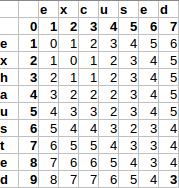
\includegraphics[scale=0.6]{image/q1.png}
	\caption{Calcul de distance}
	\label{fig1}
\end{figure}

\subsection*{Sur machine}
Nous avons ensuite calculé la distance de plusieurs mots en les comparants à des mots de classes. Cela nous permettra de les classé.

\begin{table}[h]
\centering
\resizebox{0.4\textwidth}{!}{%
\begin{tabular}{|l|l|l|l|}
\hline
       & 1     & 2     & 3     \\ \hline
abacc  & 3,2,3 & 5,4,4 & 4,4,3 \\ \hline
ccab   & 4,4,5 & 3,4,5 & 3,2,4 \\ \hline
ccbba  & 3,5,4 & 2,3,4 & 3,4,4 \\ \hline
bbaaac & 4,3,4 & 4,3,2 & 3,3,3 \\ \hline
\end{tabular}
}
\caption{Calcul de distance avec des mots de classes}
\label{my-label}
\end{table}

Voici la classification que nous obtenons, \textit{abacc} classe 1, \textit{ccab} classe 3, \textit{ccbba} classe 2 et pour \textit{bbaaac} nous avons le choix entre la classe 2 et la classe 3.

\newpage
\section*{Arbre de dérivation pour une grammaire}
\subsection*{A la main : la grammaire G}
Considérons la grammaire G:

\begin{verbatim}
- Alphabet A = {a,b,c}
- Axiome = S
- Non-terminaux = {A,B}
- Règles de production P =
    S --> cAb
    A --> aBa
    B --> aBa
    B --> cb
\end{verbatim}

\textit{G} est une grammaire algébrique puisqu'elle est de la forme $R_i:T\rightarrow x$

Cette grammaire génère le langage: \textit{L(G)} = \{c a\up{n} cb a\up{n} b $|$n$>=$1 \}. Tout d'abord on va dans S, qui impose à gauche \textit{c}, au millieu \textit{A}, et à droite \textit{b}. Dans \textit{A} nous avons, puisqu'il autorise \textit{B}, \textit{a\up{n} cb a\up{n}}. Car \textit{A} ou \textit{B} vont générer des \textit{a} à gauche et à droite.

Les arbres dérivations expliquent clairement les possibilitées de la grammaire \textit{G}.\\

Arbre de dérivation pour la chaine \textit{caacbaab}:
\begin{center}
\begin{tikzpicture}[frontier/.style={distance from root=5cm}]
\Tree[.S [.c \textit{c} ]
         [.A [.a \textit{a} ]
         	[.B [.a \textit{a} ]
         		[.B [.c \textit{c} ]
         			[.b \textit{b} ]
     			]
         		[.a \textit{a} ]
     			]
         	[.a \textit{a} ]
     		]
         [.b \textit{b} ]
     ]
\end{tikzpicture}
\end{center}

Arbre de dérivation pour la chaine \textit{cacbab}:
\begin{center}
\begin{tikzpicture}[frontier/.style={distance from root=4cm}]
\Tree[.S [.c \textit{c} ]
         [.A [.a \textit{a} ]
         		[.B [.c \textit{c} ]
         			[.b \textit{b} ]
     			]
         	[.a \textit{a} ]
     		]
         [.b \textit{b} ]
     ]
\end{tikzpicture}
\end{center}
\newpage
\subsection*{Sur machine}

Voici une grammaire de type algèbrique permettant de générer des palindromes :
\begin{verbatim}
- Alphabet Palindromes = {a,b,c,d,e,f,g,h,i,j,k,l,m,n,o,p,q,r,s,t,u,v,w,x,y,z}
- Axiome = S
- Non-terminaux = {S}
- Règles de production Palindromes =
    S --> aSa | bSb | cSc | dSd | eSe | fSf | gSg | hSh  
    S --> iSi | jSj | kSk | lSl | mSm | nSn | oSo | pSp 
    S --> qSq | rSr | sSs | tSt | uSu | vSv | wSw | xSx 
    S --> ySy | zSz | 
    S --> a | b | c | d | e | f | g | h | i | j | k 
    S --> l | m | n | o | p | q | r | s | t | u | v
    S --> w | x | y | z | 
    S --> epsilon
\end{verbatim}
\begin{center}
\begin{tikzpicture}[frontier/.style={distance from root=3cm}]
\Tree[.S [.b \textit{b} ]
         [.S [.o \textit{o} ]]
         [.b \textit{b} ]
     ]
\end{tikzpicture}
\hspace{5em}
\begin{tikzpicture}[frontier/.style={distance from root=4cm}]
\Tree[.S [.o \textit{o} ]
         [.S [.t \textit{t} ]
         	[.S [.$\epsilon$  ]]
         	[.t \textit{t} ]
         ]
         [.o \textit{o} ]
     ]
\end{tikzpicture}
\end{center}

\begin{lstlisting}
%Retourne vrai si liste vide
palindrome([]). 
%Retourne vrai si liste contient un element
palindrome([X]). 
%Parcourt iteratif du mot, on ajoute X a la tete et on test, on continue si les caracteres sont egaux
palindrome([H|T]) :- append(X,[H],T),palindrome(X)

\end{lstlisting}

\section*{Conclusion}

Dans ce tp nous avons fait quelques révisions sur la théorie des langages. Nous avons également vu une méthode nous permettant de classer des chaines de mots parmis différentes classes grâce à la distance de Levenshtein.

\end{document}